\documentclass{standalone}

\usepackage{tikz}
\usepackage{pgfplots}
\usepgfplotslibrary{statistics}
\usetikzlibrary{pgfplots.statistics}
\usepackage{etoolbox}

\newtoggle{label}
\togglefalse{label}

\pgfplotsset{compat=1.12}

\begin{document}
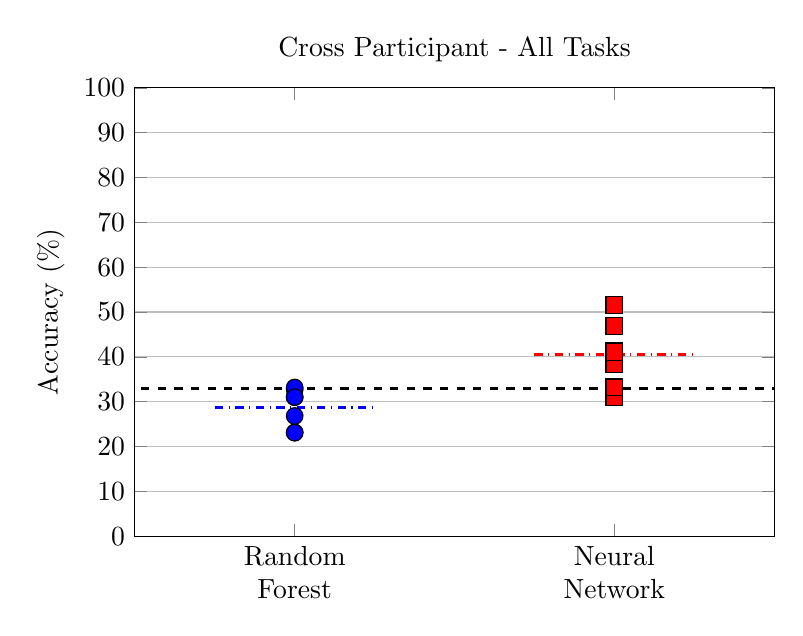
\begin{tikzpicture}
\begin{axis}[
	ymajorgrids,
	width=0.8\textwidth,
	height=0.6\textwidth,
	scatter/classes= {
		a={mark=*, fill=blue, draw=black, mark size=3},
		b={mark=square*, fill=red, draw=black, mark size=3}
	},
	ymin=0,
	ymax=100,
	xmin = .5, 
	xmax=2.5,
	ytick={0,10,...,100},
	xtick={1,2},
	xticklabel style={align=center},
	xticklabels={Random\\Forest, Neural\\Network},
	title=Cross Participant - All Tasks, 
	ylabel=Accuracy (\%)]

\addplot+[ mark=None, dashed, black, line width = 1pt ]
	coordinates {
	(0, 33)
	(3, 33)	
};

	% Random Forest
	\addplot+[ scatter,
			only marks,
			scatter src=explicit symbolic]
	coordinates {
			(1, 32.70) [a]
			(1, 23.14) [a]
			(1, 23.08) [a]
			(1, 31.03) [a]
			(1, 33.17) [a]
			(1, 31.02) [a]
			(1, 26.82) [a]
};

% RF Mean
	\addplot+[ mark=None, dashdotted, blue, line width = 1pt ] 
	coordinates {
		(0.75, 28.70)
		(1.25, 28.70)
};

	% ANN
	\addplot+[ scatter,
			only marks,
			scatter src=explicit symbolic]
	coordinates {
			(2, 41.33) [b]
			(2, 30.92) [b]
			(2, 33.21) [b]
			(2, 38.34) [b]
			(2, 51.57) [b]
			(2, 46.89) [b]
			(2, 41.08) [b]
};

% ANN Mean
	\addplot+[ mark=None, dashdotted, red, line width = 1pt ] 
	coordinates {
		(1.75, 40.47)
		(2.25, 40.47)
};


\end{axis}
\end{tikzpicture}

\end{document}
















